\documentclass[border=3pt,tikz]{standalone}

\usepackage{amsmath}
\DeclareMathOperator{\asinh}{asinh}
% taken from
% https://tex.stackexchange.com/questions/153957/drawing-neural-network-with-tikz
\usepackage{tikz}
\usepackage{etoolbox} % for \ifnumcomp
\usepackage{listofitems} % for \readlist to create arrays
\usepackage[T1]{fontenc}
\usetikzlibrary{math} 
\definecolor{myorange}{HTML}{EC6500}
\definecolor{myred}{HTML}{E6001A}
\definecolor{myblue}{HTML}{005AA9}
\definecolor{mygreen}{HTML}{009D81}
\definecolor{TUD4c}{HTML}{7FAB16}
\definecolor{TUD2b}{HTML}{0083CC}
\definecolor{TUD4b}{HTML}{99C000}
\definecolor{TUD7b}{HTML}{F5A300}
\definecolor{mydarkorange}{HTML}{A94913}
\definecolor{mydarkred}{HTML}{961C26}
\definecolor{mydarkblue}{HTML}{243572}
\definecolor{mydarkgreen}{HTML}{00715E}
%\colorlet{myred}{red!80!black}
%\colorlet{myblue}{blue!80!black}
%\colorlet{mygreen}{green!60!black}
%\colorlet{mydarkred}{myred!40!black}
%\colorlet{mydarkblue}{myblue!40!black}
%\colorlet{mydarkgreen}{mygreen!40!black}
\tikzstyle{node}=[very thick,circle,draw=myblue,minimum size=22,inner sep=0.5,outer sep=0.6]
\tikzstyle{connect}=[-,thick,black]
%\tikzset{>=latex} % for LaTeX arrow head
%\tikzstyle{connect}=[->,thick,black,shorten >=1]
\tikzset{ % node styles, numbered for easy mapping with \nstyle
%	node 1/.style={node,mydarkgreen,draw=mygreen,fill=mygreen!20},
	node 1/.style={node,black,draw=black,fill=TUD2b},
	node 2/.style={node,black,draw=black,fill=TUD4b},
	node 3/.style={node,black,draw=black,fill=TUD4b},
	node 4/.style={node,black,draw=black,fill=TUD7b},
	node 5/.style={node,black,draw=black},
	node 6/.style={node,black,draw=black},
	node 7/.style={node,black,draw=black},
}
\def\nstyle{int(\lay)} % each layer has its own style
%\def\nstyle{int(  \lay<\Nnodlen-1?min(4,\lay)  :  (\lay==\Nnodlen-1?5:6)  )} % map layer number onto 1, 2, 3, or 4

\usepackage{helvet}
\usepackage[outline]{contour}
\contourlength{3.0pt}

\newcommand{\Minus}{
	\mathord{
		\begin{tikzpicture}[baseline=0ex, line width=1.5, scale=0.13]
			\draw (0,0.5) -- (1,0.5);
		\end{tikzpicture}
	}
}

\begin{document}
	
	
	% NEURAL NETWORK
	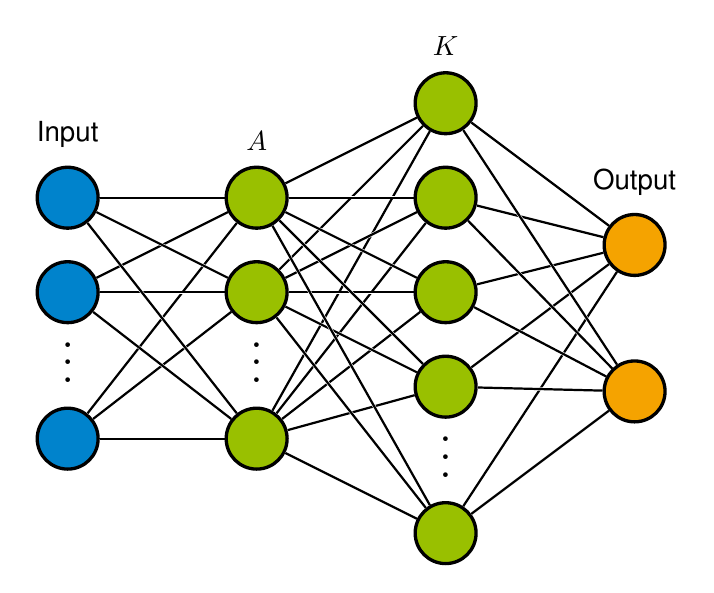
\begin{tikzpicture}[x=2.4cm,y=1.2cm]
		\readlist\Nnod{3,3,5,2} % array of number of nodes per layer
		\readlist\Nstr{,n+1,m,2} % array of string number of nodes per layer
		\readlist\Cstr{,,,} % array of coefficient symbol per layer
%		\readlist\Cstr{p,\ln p,,,,$$\dot{s}$$}
		\def\yshift{0.55} % shift last node for dots
		
		% LOOP over LAYERS
		\foreachitem \N \in \Nnod{
			\def\lay{\Ncnt} % alias of index of current layer
			\pgfmathsetmacro\prev{int(\Ncnt-1)} % number of previous layer
			\foreach \i [evaluate={\c=int(\i==\N); \y=\N/2-\i-\c*\yshift;
				\x=\lay; \n=\nstyle;
				\index=(\i<\N?int(\i):"\Nstr[\n]");
				\indexshifted=(\i<\N?int(\i-1):"\Nstr[\n]");}] in {1,...,\N}{ % loop over nodes
				% NODES
				% -----
				
				% layer 1 is special
				\ifnum \lay=1
					\ifnum \i=1
						\node[node \n] (N\lay-\i) at (\x,\y) {};%$T^{-1}$
					\else
						\node[node \n] (N\lay-\i) at (\x,\y) {};%$\strut\Cstr[\n]_{\indexshifted}$
					\fi
				\fi
				% layer 2 and 3 is not labeled
				\ifnum \lay=2
					\node[node \n] (N\lay-\i) at (\x,\y) {};
				\fi
				\ifnum \lay=3
					\node[node \n] (N\lay-\i) at (\x,\y) {};
				\fi
				\ifnum \lay=4
					\ifnum \i=1
						\node[node \n] (N\lay-\i) at (\x,\y) {};%$\ln r^+$
					\fi
					\ifnum \i=2
						\node[node \n] (N\lay-\i) at (\x,\y) {};%$\ln r^-$
					\fi
				\fi


				
				
				
				% CONNECTIONS
				\ifnumcomp{\lay}{>}{1}{ % connect to previous layer
					{
						\foreach \j in {1,...,\Nnod[\prev]}{ % loop over nodes in previous layer
							\draw[white,line width=1.2,shorten >=1] (N\prev-\j) -- (N\lay-\i);
							\draw[connect] (N\prev-\j) -- (N\lay-\i);
						}
						\ifnum \lay=\Nnodlen
	%					\draw[connect] (N\lay-\i) --++ (0.5,0); % arrows out
						\fi
					}
				}{
					%{\draw[connect] (0.5,\y) -- (N\lay-\i);} % arrows in
				}
				
			}
			\ifnumcomp{\N}{<}{3}{} % no dots
			\path (N\lay-\N) --++ (0,1+\yshift) node[midway,scale=1.6] {$\vdots$}; % dots
		}
		
		% LABELS
		\node[above=3,align=center,black,font=\fontfamily{phv}\selectfont] at (N1-1.90) {Input};
		\node[above=2,align=center,black,font=\fontfamily{phv}\selectfont] at (N2-1.90) {$A$};
		\node[above=2,align=center,black,font=\fontfamily{phv}\selectfont] at (N3-1.90) {$K$};
		\node[above=3,align=center,black,font=\fontfamily{phv}\selectfont] at (N4-1.90) {Output};
		
	\end{tikzpicture}
	
	
\end{document}